\documentclass[10pt,t,aspectratio=169]{beamer}

\usetheme[progressbar=frametitle]{moloch}

%\usepackage{helvet}
%\usepackage[sfdefault,light]{FiraSans}
\usepackage[sfdefault]{inter}

\usepackage[T1]{fontenc}
\usepackage[latin9]{inputenc}
\usepackage{amsmath}
\usepackage{amsthm}
\usepackage{amssymb}
\PassOptionsToPackage{no-math}{fontspec}
\usepackage{graphicx} 
\usepackage{hyperref} 
\usepackage{multirow} 
\usepackage{xspace}
\usepackage{booktabs}
\usepackage{dcolumn}

\setbeamercolor{normal text}{fg=mDarkTeal,bg=white}
\definecolor{cardinalred}{rgb}{0.549, 0.082, 0.082}
\setbeamercolor{progress bar}{ fg = white }
\setbeamercolor{title separator}{ fg = cardinalred}
\setbeamercolor{progress bar in section page}{ fg = cardinalred }

\newtheorem{proposition}{Proposition} 

\title{O Praeclarum Titulum}
\subtitle{Lorem ipsum dolor}
% \date{\today}
\date{}
\author{Author 1 (Affiliation) \\
        Author 2 (Affiliation)}

\begin{document}

\maketitle

\begin{frame}{Motivation}

    motivation

\end{frame}

\begin{frame}{This paper}

    this paper
  
\end{frame}

\section{Background}

\begin{frame}{xxx}

    xxx
  
\end{frame}

\section{Data}

\begin{frame}{xxx}

    xxx
  
\end{frame}

\section{Results}

\begin{frame}{City Fuel Economy Plot In Logs}

	\begin{figure}[!htp]
    	\centering
   	 	\caption{\bf{City Fuel Economy Plot In Logs}}
   		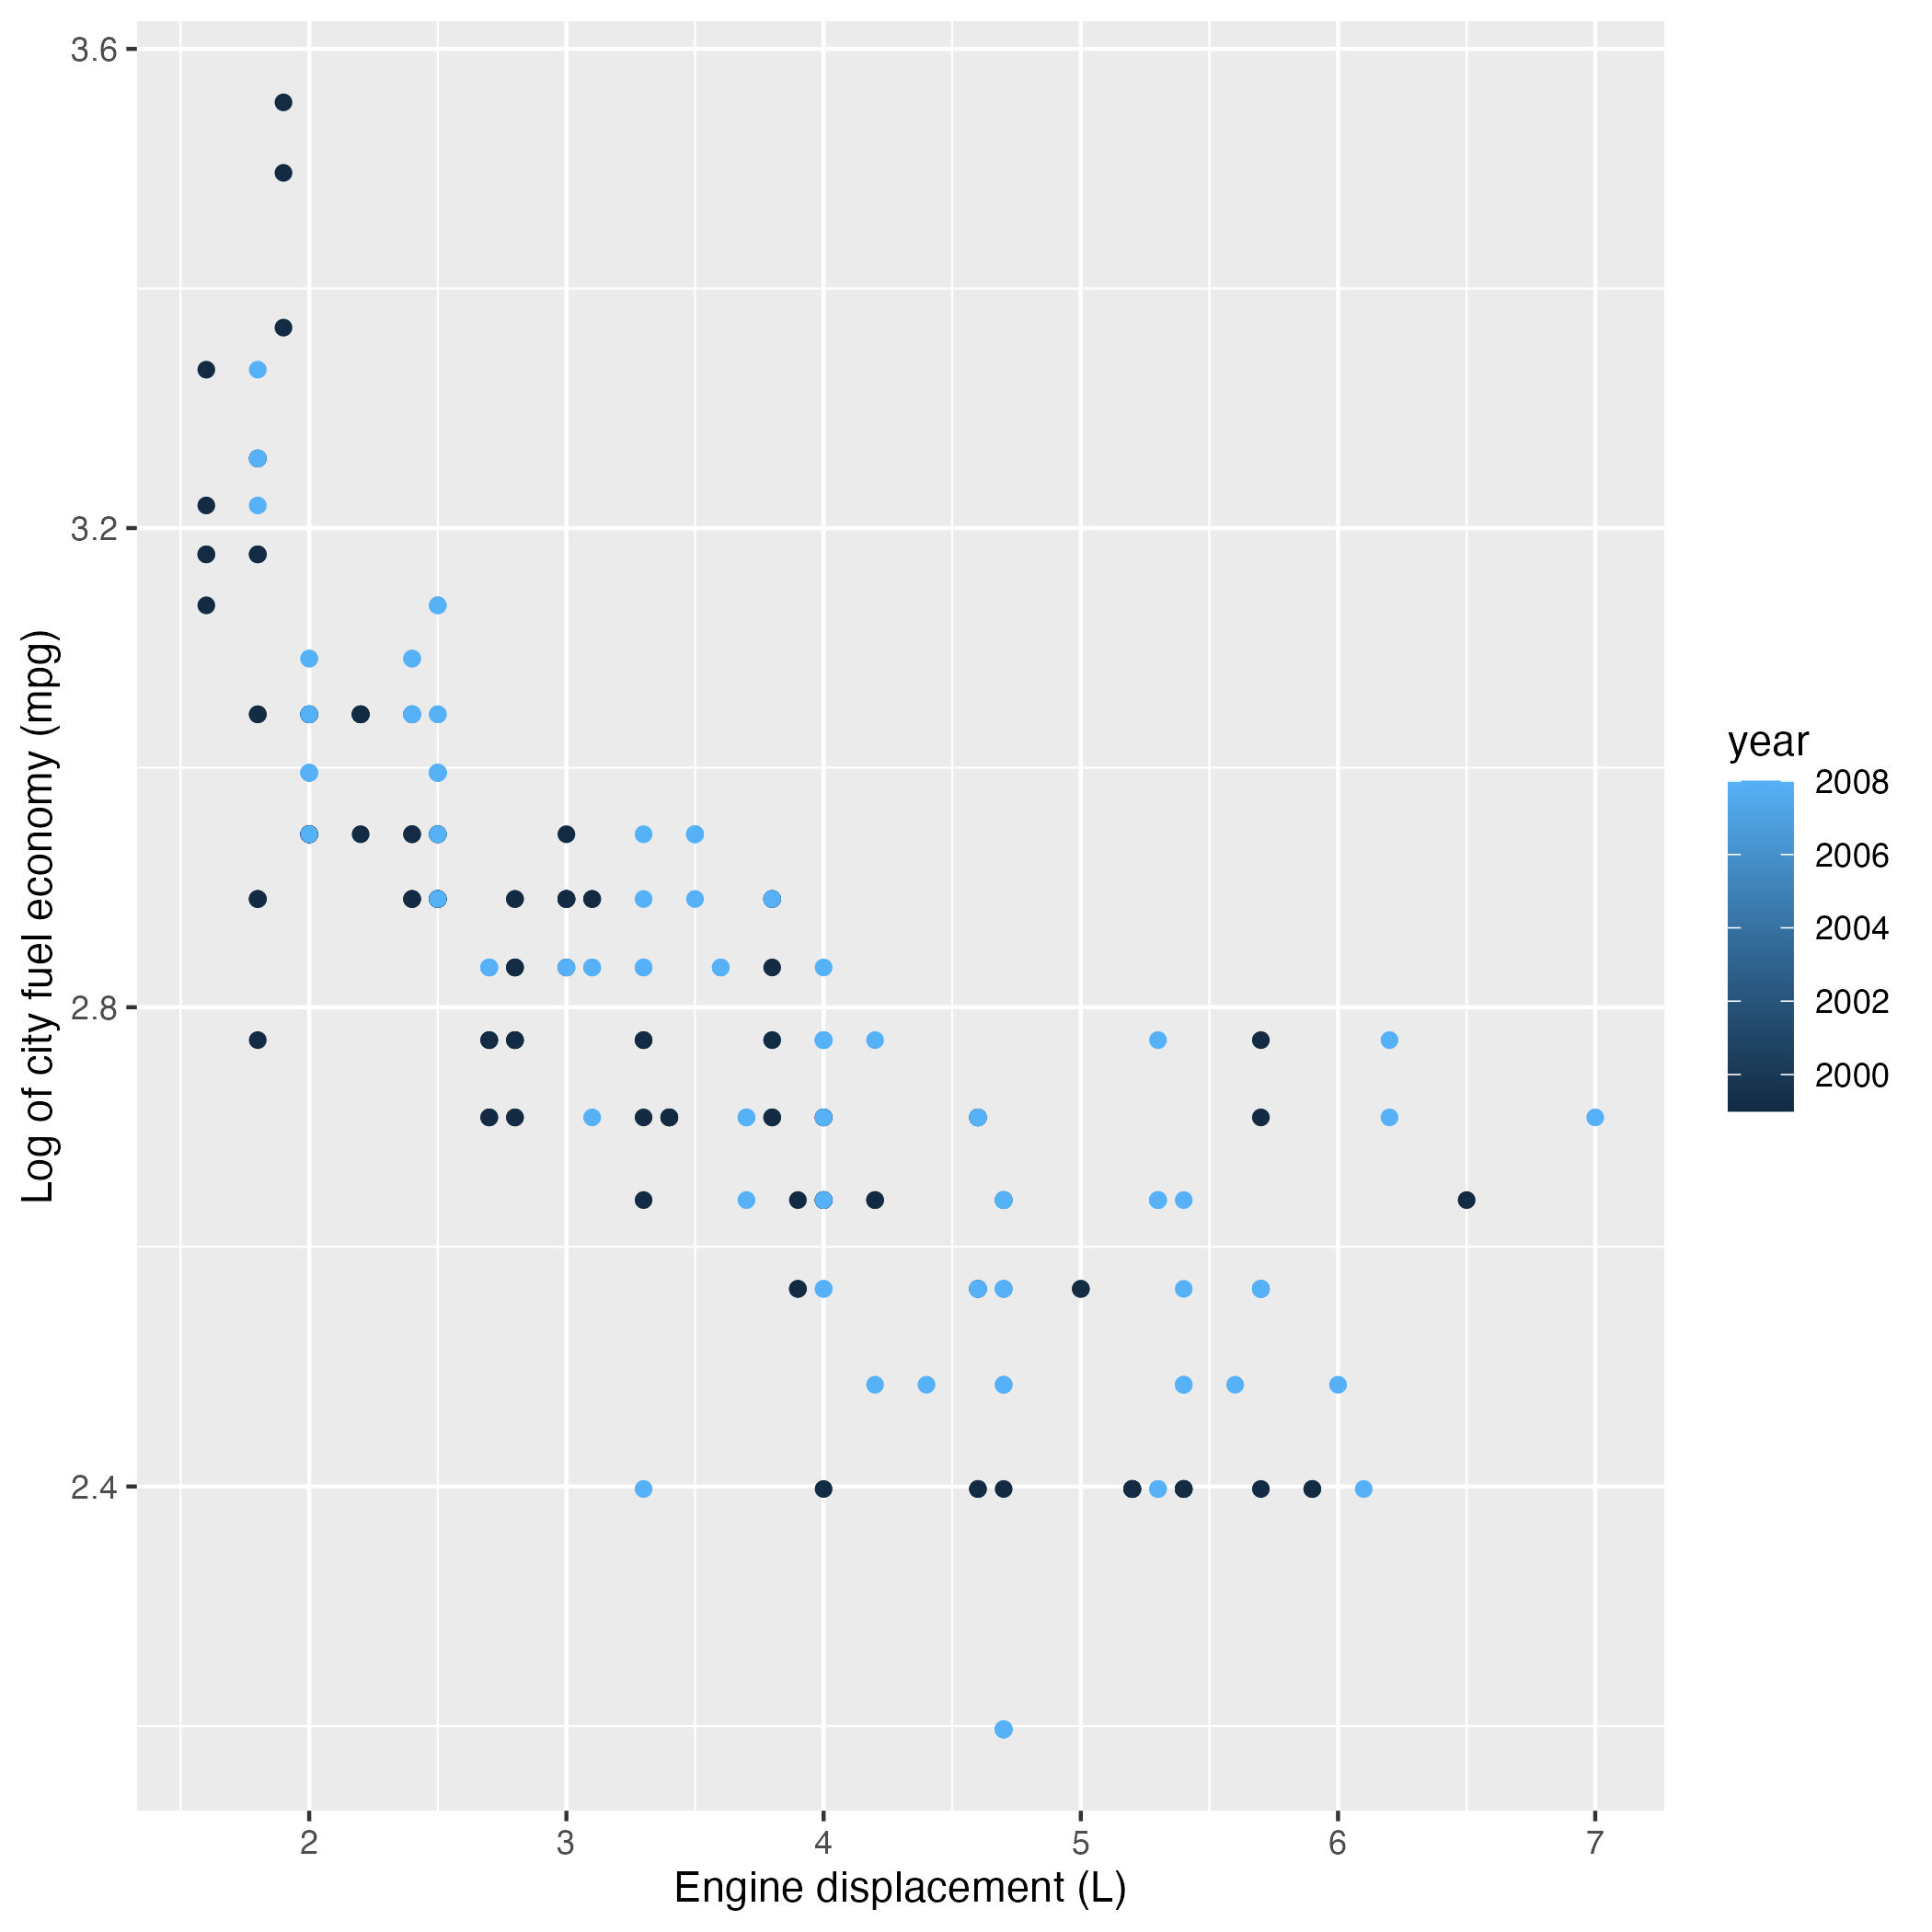
\includegraphics[scale=0.08]{../input/figure_city.jpg}
	\end{figure}
  
\end{frame}

\begin{frame}{Regression Table With Clustered SEs}
  \centering
  \textbf{Table 1: Regression Results with Clustered SEs}
  \vspace{0.3cm}
  \resizebox{\textwidth}{!}{
% Table created by stargazer v.5.2.3 by Marek Hlavac, Social Policy Institute. E-mail: marek.hlavac at gmail.com
% Date and time: Mon, Jul 14, 2025 - 03:18:08 PM
% Requires LaTeX packages: dcolumn 
\begin{tabular}{@{\extracolsep{5pt}}lD{.}{.}{-3} D{.}{.}{-3} D{.}{.}{-3} } 
\\[-1.8ex]\hline 
\hline \\[-1.8ex] 
 & \multicolumn{3}{c}{\textit{Dependent variable:}} \\ 
\cline{2-4} 
\\[-1.8ex] & \multicolumn{3}{c}{Engine displacement (L)} \\ 
\\[-1.8ex] & \multicolumn{1}{c}{(1)} & \multicolumn{1}{c}{(2)} & \multicolumn{1}{c}{(3)}\\ 
\hline \\[-1.8ex] 
 City fuel economy (mpg) & -0.242^{***} &  & -0.233^{*} \\ 
  & (0.022) &  & (0.125) \\ 
  & & & \\ 
 Highway fuel economy (mpg) &  & -0.166^{***} & -0.007 \\ 
  &  & (0.005) & (0.077) \\ 
  & & & \\ 
 Constant & 7.558^{***} & 7.368^{***} & 7.565^{***} \\ 
  & (0.522) & (0.307) & (0.450) \\ 
  & & & \\ 
\hline \\[-1.8ex] 
Observations & \multicolumn{1}{c}{234} & \multicolumn{1}{c}{234} & \multicolumn{1}{c}{234} \\ 
R$^{2}$ & \multicolumn{1}{c}{0.638} & \multicolumn{1}{c}{0.587} & \multicolumn{1}{c}{0.638} \\ 
Adjusted R$^{2}$ & \multicolumn{1}{c}{0.636} & \multicolumn{1}{c}{0.585} & \multicolumn{1}{c}{0.635} \\ 
Residual Std. Error & \multicolumn{1}{c}{0.779 (df = 232)} & \multicolumn{1}{c}{0.832 (df = 232)} & \multicolumn{1}{c}{0.781 (df = 231)} \\ 
\hline 
\hline \\[-1.8ex] 
\textit{Note:}  & \multicolumn{3}{r}{$^{*}$p$<$0.1; $^{**}$p$<$0.05; $^{***}$p$<$0.01} \\ 
\end{tabular} 
}
\end{frame}


\section{Conclusion}

\begin{frame}{xxx}

    xxx
  
\end{frame}

\end{document}
